% Options for packages loaded elsewhere
\PassOptionsToPackage{unicode}{hyperref}
\PassOptionsToPackage{hyphens}{url}
%
\documentclass[
]{book}
\usepackage{amsmath,amssymb}
\usepackage{lmodern}
\usepackage{ifxetex,ifluatex}
\ifnum 0\ifxetex 1\fi\ifluatex 1\fi=0 % if pdftex
  \usepackage[T1]{fontenc}
  \usepackage[utf8]{inputenc}
  \usepackage{textcomp} % provide euro and other symbols
\else % if luatex or xetex
  \usepackage{unicode-math}
  \defaultfontfeatures{Scale=MatchLowercase}
  \defaultfontfeatures[\rmfamily]{Ligatures=TeX,Scale=1}
\fi
% Use upquote if available, for straight quotes in verbatim environments
\IfFileExists{upquote.sty}{\usepackage{upquote}}{}
\IfFileExists{microtype.sty}{% use microtype if available
  \usepackage[]{microtype}
  \UseMicrotypeSet[protrusion]{basicmath} % disable protrusion for tt fonts
}{}
\makeatletter
\@ifundefined{KOMAClassName}{% if non-KOMA class
  \IfFileExists{parskip.sty}{%
    \usepackage{parskip}
  }{% else
    \setlength{\parindent}{0pt}
    \setlength{\parskip}{6pt plus 2pt minus 1pt}}
}{% if KOMA class
  \KOMAoptions{parskip=half}}
\makeatother
\usepackage{xcolor}
\IfFileExists{xurl.sty}{\usepackage{xurl}}{} % add URL line breaks if available
\IfFileExists{bookmark.sty}{\usepackage{bookmark}}{\usepackage{hyperref}}
\hypersetup{
  pdftitle={TILM 3701 - Tilastotiede ja Data 2022},
  pdfauthor={Koonneet; Henri Nyberg; Roope Rihtamo},
  hidelinks,
  pdfcreator={LaTeX via pandoc}}
\urlstyle{same} % disable monospaced font for URLs
\usepackage{longtable,booktabs,array}
\usepackage{calc} % for calculating minipage widths
% Correct order of tables after \paragraph or \subparagraph
\usepackage{etoolbox}
\makeatletter
\patchcmd\longtable{\par}{\if@noskipsec\mbox{}\fi\par}{}{}
\makeatother
% Allow footnotes in longtable head/foot
\IfFileExists{footnotehyper.sty}{\usepackage{footnotehyper}}{\usepackage{footnote}}
\makesavenoteenv{longtable}
\usepackage{graphicx}
\makeatletter
\def\maxwidth{\ifdim\Gin@nat@width>\linewidth\linewidth\else\Gin@nat@width\fi}
\def\maxheight{\ifdim\Gin@nat@height>\textheight\textheight\else\Gin@nat@height\fi}
\makeatother
% Scale images if necessary, so that they will not overflow the page
% margins by default, and it is still possible to overwrite the defaults
% using explicit options in \includegraphics[width, height, ...]{}
\setkeys{Gin}{width=\maxwidth,height=\maxheight,keepaspectratio}
% Set default figure placement to htbp
\makeatletter
\def\fps@figure{htbp}
\makeatother
\setlength{\emergencystretch}{3em} % prevent overfull lines
\providecommand{\tightlist}{%
  \setlength{\itemsep}{0pt}\setlength{\parskip}{0pt}}
\setcounter{secnumdepth}{5}
\usepackage{booktabs}
\usepackage{amsthm}
\makeatletter
\def\thm@space@setup{%
  \thm@preskip=8pt plus 2pt minus 4pt
  \thm@postskip=\thm@preskip
}
\makeatother

\usepackage{color}
\usepackage{framed}
\setlength{\fboxsep}{.8em}

\usepackage{tcolorbox}

\newtcolorbox{blackbox}{
  colback=black,
  colframe=orange,
  coltext=white,
  boxsep=5pt,
  arc=4pt}

%\newenvironment{infobox}[1]
%  {\begin{itemize}
%    \renewcommand{\labelitemi}{
%    \raisebox{-.7\height}[0pt][0pt]{
%      {\setkeys{Gin}{width=3em,keepaspectratio}
%        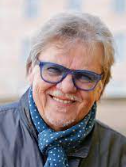
\includegraphics{images/mikko.PNG}}
%    }
%  }
%  \setlength{\fboxsep}{1em}
%  \begin{blackbox}
%  \item}
%  {
%  \end{blackbox}
%  \end{itemize}
%}
\usepackage{awesomebox}
\ifluatex
  \usepackage{selnolig}  % disable illegal ligatures
\fi
\usepackage[]{natbib}
\bibliographystyle{apalike}

\title{TILM 3701 - Tilastotiede ja Data 2022}
\author{Koonneet \and Henri Nyberg\footnote{Turun Yliopisto, matematiikan ja tilastotieteen laitos, \href{mailto:henri.nyberg@utu.fi}{\nolinkurl{henri.nyberg@utu.fi}}} \and Roope Rihtamo\footnote{Turun Yliopisto, matematiikan ja tilastotieteen laitos, \href{mailto:roope.rihtamo@utu.fi}{\nolinkurl{roope.rihtamo@utu.fi}}}}
\date{2022-08-22}

\begin{document}
\maketitle

{
\setcounter{tocdepth}{1}
\tableofcontents
}
\hypertarget{tilastotiede-ja-kurssin-idea}{%
\chapter*{Tilastotiede ja kurssin idea}\label{tilastotiede-ja-kurssin-idea}}
\addcontentsline{toc}{chapter}{Tilastotiede ja kurssin idea}

\begin{itemize}
\tightlist
\item
  Tämän tilastotieteen ensimmäisen kurssin ideana on (ainakin)

  \begin{itemize}
  \tightlist
  \item
    Esitellä ja johdatella \textbf{tilastolliseen ja tieteelliseen ajatteluun} ja sen hyödyntämiseen eri tyyppisissä tutkimusongelmissa.
  \item
    Esitellä tilastotieteen roolia \textbf{empiirisen tutkimusaineiston keräämisessä ja analyysissä} sekä tarkastella tieteentekemisen ja tilastotieteen suhdetta.
  \item
    Pohtia \textbf{tilastotieteen olemusta tieteenalana} ja tarkastella tilastotieteen ja datatieteiden (data sciencen) samankaltaisuuksia ja eroja.
  \item
    Pohtia \textbf{sattuman ja satunnaisuuden roolia} jokapäiväisessä elämässä ja erityisesti osana tieteellistä tutkimusprosessia.
  \item
    Oppia tilastotieteen peruskäsitteitä ja (tilastollisen) tutkimuksenteon alkeita ja siihen liittyviä mahdollisia ongelmia esimerkiksi tilastollisten aineistojen keräämisessä.
  \item
    Oppia tilastollisten aineistojen \textbf{kuvaamisen ja käsittelyn} alkeita sekä tilasto(tieteellisen)llisen \textbf{mallintamisen} ja \textbf{koeasetelmien} peruskäsitteitä.
  \end{itemize}
\end{itemize}

\vspace{0.75cm}

\begin{itemize}
\tightlist
\item
  Kurssilla käsitellään myös \textbf{tilastollisen päättelyn} peruskäsitteitä ja perusteita kuten

  \begin{itemize}
  \tightlist
  \item
    Mitä on \textbf{todennäköisyys} ja miten sen tulkitaan tilastotieteessä sekä laajemmin tieteessä. Erityisesti tilastotieteen osalta keskiössä on tämän kurssin osalta \textbf{satunnaismuuttujat} sekä niihin liitettävät käsitteet

    \begin{itemize}
    \tightlist
    \item
      \textbf{Odotusarvo}, \textbf{varianssi} ja kahden (tai useamman) satunnaismuuttujan \textbf{korrelaatio}.
    \item
      Satunnaismuuttujien \textbf{todennäköisyysjakaumien} perusteita ja niiden yhteyksiä mm. normaalijakaumaan ja muutamiin muihin keskeisiin jakaumiin.
    \item
      Tilastollinen malli työkaluna satunnaismuuttujien formaalissa mallintamisessa ja päättelyssä. Tilastollisen malliin liittyy (usein) \textbf{parametreja} joihin tilastollinen päättely kohdistuu.
    \item
      Tilastollisten mallien \textbf{estimoinnin} perusidea, eli miten tilastollisen mallin parametreille muodostetaan arvot käytettävissä olevan aineiston pohjalta. Esimerkiksi: mitä tarkoittaa tilastollisen mallin parametrin \textbf{estimaattori} ja sen \textbf{harhattomuus}?
    \item
      Alustavia tarkasteluja tilastollisen mallin uskottavuuden käsitteelle ja \textbf{luottamusväleille} tilastollisen mallin estimoiduille parametreille.
    \end{itemize}
  \end{itemize}
\end{itemize}

\vspace{0.75cm}

\begin{itemize}
\tightlist
\item
  Toinen kurssin keskeisistä teemoista on tarkastella tieteellistä tutkimusprosessia teoriassa ja käytännössä. Tämä sisältää mm. seuraavia aiheita (joita siis käsitellään tällä kurssilla päällisin puolin ja varsin yleisestä näkökulmasta katsoen): tarkemmat yksityiskohdat jäävät tätä kurssia seuraavien tilastotieteen kurssien aihepiireiksi):

  \begin{itemize}
  \tightlist
  \item
    \textbf{Tutkimusongelman} asettaminen: mitä halutaan tutkia?\\
  \item
    Tutkimusongelman täsmentäminen ja \textbf{tutkimusstrategian} laatiminen: millä keinoin asetettuun tutkimusongelmaan voidaan vastata?
  \item
    \textbf{Tutkimusaineiston} (tai vain lyhyemmin \textbf{aineiston} eli \textbf{datan}) kerääminen

    \begin{itemize}
    \tightlist
    \item
      \textbf{Aineiston ennakkoehdot}: mitkä ehdot tulee täyttyä, jotta asetettuun tutkimusongelmaan voidaan vastata?
    \item
      \textbf{Otanta} (ja mittaaminen): miten tutkimusaineisto kerätään niin, että se täyttää aineiston ennakkoehdot? Erilaisissa tutkimuksissa käytetään erilaisia aineistoja kuten:

      \begin{itemize}
      \tightlist
      \item
        Survey- ja rekisteriaineistot
      \item
        Havaintoarvojen välistä korrelaatiota esiintyy mm. aikasarja-aineistojen tai pitkittäisaineistojen tapauksessa
      \end{itemize}
    \end{itemize}
  \end{itemize}
\item
  \textbf{Aineiston kuvaaminen}: minkälaista aineistoa on kerätty ja vastaako se ennakkoehtoja?
\item
  \textbf{Aineiston analyysin} lähtökohtia

  \begin{itemize}
  \tightlist
  \item
    Mitä tilastollista mallia/malleja käytetään?
  \item
    Mitä tarkoitetaan mallien tuntemattomien parametrien arvojen estimoinnilla?
  \item
    Tilastollinen päättely (estimointitulosten pohjalta)
  \end{itemize}
\item
  \textbf{Johtopäätelmien} tekeminen tilastollisen päättelyn pohjalta: saatiinko tutkimusongelmaan vastaus ja kuinka luotettava saatu vastaus on?
\end{itemize}

\hypertarget{tilastotieteen-asema-tutkimusyhteisuxf6n-ulkopuolella}{%
\section*{Tilastotieteen asema tutkimusyhteisön ulkopuolella}\label{tilastotieteen-asema-tutkimusyhteisuxf6n-ulkopuolella}}
\addcontentsline{toc}{section}{Tilastotieteen asema tutkimusyhteisön ulkopuolella}

\begin{itemize}
\tightlist
\item
  Tilastotiede on oppiaineena usein varsin tuntematon toisen asteen opinnoista valmistuneelle, sillä sitä ei juurikaan opeteta lukioissa tai ammattikouluissa huolimatta sen keskeisestä ja kasvavasta roolista tiedemaailman kentillä.
\item
  Tiedeyhteisön ulkopuolellakin \textbf{tilastotiedettä ja tilastotieteilijöitä arvostetaan laajalti}.
\item
  \textbf{Tilastotiede onkin nostanut profiiliaan viimeisten vuosikymmenien aikana} tietoteknisen kehityksen tuotua laajat tietoaineistot ja kehittyneet laskennalliset menetelmät lähes jokaisen kansalaisen saataville.
\item
  Tämä ``datavallankumous'' näkyy tilastotieteilijöiden kysynnässä työmarkkinoilla: erilaisten aineistojen määrän lisääntyessä kasvaa myös kysyntä työntekijöistä, jotka osaavat ammatitaitoisesti käsitellä, tulkita ja mallintaa tilastollisia aineistoja.
\item
  Ei siis liene ihmekään, että erilaisten ``data''-alkuisten työpaikkojen, kuten \textbf{datatieteilijä} (eng. \textbf{data scientist}) tai \textbf{data-analyytikko} ( \textbf{data-analyst}) määrä on kasvanut voimakkaasti jo pidempään. Kaikkia tieto- ja datainensiivisten ammattien tekijöitä yhdistää yksi tekijä: \textbf{heidän tulee hallita ja osata tilastotiedettä!} Karkeistettuna mitä paremmin ja enemmän (laajemmin), sen parempi palkka ja monipuolisemmat työtehtävät!
\end{itemize}

\hypertarget{kurssin-luonne-tilastotieteen-ja-datatieteendata-analytiikan-opintojen-esittelijuxe4nuxe4}{%
\section*{Kurssin luonne tilastotieteen (ja datatieteen/data-analytiikan) opintojen esittelijänä}\label{kurssin-luonne-tilastotieteen-ja-datatieteendata-analytiikan-opintojen-esittelijuxe4nuxe4}}
\addcontentsline{toc}{section}{Kurssin luonne tilastotieteen (ja datatieteen/data-analytiikan) opintojen esittelijänä}

Kurssin mittaan esitellään tilastotieteen perusteiden lisäksi \textbf{miten TY:ssa tilastotieteen opinnoissa syvennytään} tällä kurssilla esiteltäviin menetelmiin, aineistotyyppeihin ja mallinnuskokonaisuuksiin.

\hypertarget{luku2}{%
\chapter{Tieteellinen tieto, tilastot ja arkitieto yhteiskunnassa}\label{luku2}}

Tässä luvussa tarkastellaan tieteen ja tieteellisen tutkimusprosessin luonnetta erityisesti uuden \textbf{tutkitun} tiedon tuottamisen näkökulmasta. Tiedelukutaidon merkitys on kasvanut nyky-yhteiskunnassa, kun tiedejulkaisujen saavutettavuus ja tunnettuus on lisääntynyt mm. tieteen popularisoinnin ja median laajemman tiedeuutisoinnin vuoksi. Voidakseen ymmärtää ja arvioida kriittisesti tiedeuutisia tulee lukijan olla tietoinen tieteellisen tutkimuksen luonteesta: miten tutkimusartikkeleja luetaan, mitä niiltä voidaan odottaa ja minkälaiset tulokset ovat uskottavia. \textbf{Tilastotiede näyttelee keskeistä roolia lähes kaikessa tutkimuksessa ja erityisesti erilaisten tutkimuskysymysten ja niitä vastaavien hypoteesien testauksessa}. Aloitetaankin kurssin oppimateriaalin käsittely määrittelemällä ensimmäinen tilastotieteen perustermi: hypoteesi.

\begin{noteblock}{}

\textbf{Hypoteesi}

\begin{itemize}
\tightlist
\item
  Hypoteesi tarkoittaa (tausta)teorioista johdettua tai aikaisemman tutkimuksen perusteella esitettyä ennakoitua ratkaisua tai selitystä tutkittavaan ongelmaan.
\item
  Hypoteesi ilmaistaan väitteenä, jonka paikkansapitävyyttä halutaan tutkia
\item
  Kokeelliset tiedot voivat osoittaa hypoteesin vääräksi
\item
  Nollahypoteesi vastaa tavallisesti tyypillistä, odotettavissa olevaa tulosta, esimerkiksi ettei kahden mitatun ilmiön välillä ole yhteyttä tai että tietty hoito on tehotonta
\item
  Nollahypoteesia ei todisteta (``hyväksytä''), vaan voidaan ainoastaan sanoa, ettei aineisto tarjoa todistusaineistoa (``evidenssiä'') nollahypoteesin hylkäämiselle -- ts. sille tulemalle, että emme hylkää nollahypoteesia.
\item
  Vastahypoteesi sisältää usein mielenkiinnon kohteena olevan tapahtuman, kuten ``on eroa'' tai ``on vaikutusta''
\item
  Tutkijoilla on usein taipumus jättää julkaisematta tutkimustuloksia, joissa nollahypoteesi jää voimaan. Yleensä tämä tilanne syntyy, kun lopputulos ei eroa jo aikaisemmin otaksutusta. (Toki ajoittain tilanne on myös toisinpäin)
\end{itemize}

\end{noteblock}

Tähän joku esimerkki vielä?

\hypertarget{tieteellinen-ajattelu-tietoyhteiskunnan-perustana}{%
\section{Tieteellinen ajattelu tietoyhteiskunnan perustana}\label{tieteellinen-ajattelu-tietoyhteiskunnan-perustana}}

Kesken vielä.

\hypertarget{tilastojen-yleisestuxe4-roolista-yhteiskunnassa}{%
\section{Tilastojen yleisestä roolista yhteiskunnassa}\label{tilastojen-yleisestuxe4-roolista-yhteiskunnassa}}

Kesken vielä.

\hypertarget{mituxe4-on-tiede}{%
\section{Mitä on tiede?}\label{mituxe4-on-tiede}}

Kesken vielä.

\hypertarget{mituxe4-on-tutkimus}{%
\section{Mitä on tutkimus?}\label{mituxe4-on-tutkimus}}

Kesken vielä.

\hypertarget{tieteellisen-menetelmuxe4n-kriteereituxe4}{%
\section{Tieteellisen menetelmän kriteereitä}\label{tieteellisen-menetelmuxe4n-kriteereituxe4}}

Kesken vielä.

\hypertarget{tieteellinen-tutkimuksen-vaiheet-ja-tulosten-julkaiseminen}{%
\section{Tieteellinen tutkimuksen vaiheet ja tulosten julkaiseminen}\label{tieteellinen-tutkimuksen-vaiheet-ja-tulosten-julkaiseminen}}

Tieteellinen tutkimus ja asiantuntijatyö tuottavat valtavan määrän perusteltua, luotettavaa tutkimustietoa. Ks. tarkemmin tieteellisestä julkaisemisesta linkin tapauksessa erityisesti yhteiskuntatieteiden alalla, mutta perusperiaatteet pätevät myös muiden tieteenalojen tapauksessa

\vspace{0.5cm}

\url{https://blogs.uef.fi/tiedonhaku-yhteiskuntatiede/tieteelliset-julkaisut/}

\vspace{0.5cm}

Vastuullisen tieteen
\vspace{0.5cm}

\url{https://vastuullinentiede.fi/fi/julkaiseminen}

\vspace{0.5cm}

\noindent artikkelit tarjoavat tietoa siitä, kuinka tutkittua tietoa tuotetaan, julkaistaan ja arvioidaan luotettavasti ja yhteisesti hyväksytyllä tavalla. Jotta tiede vaikuttaa koko yhteiskunnan hyväksi, toiminnan on oltava vastuullista tutkimuksen jokaisessa vaiheessa.

\begin{itemize}
\item
  Julkisuus ja avoimuus tekevät tutkimuksesta tiedettä.
\item
  Tiedeviestintä on tiedeyhteisöjen sisäistä ja ulkoista tiedonvälitystä ja vuorovaikutusta. Tutkimuksesta viestiminen ei ole vain tutkimustuloksista viestimistä. Vastuullinen tiedeviestintä lisää luottamusta tieteelliseen tietoon.
\item
  Tieteellinen julkaiseminen on tutkijoille tärkeä meritoitumisen tapa, ja siksi on tärkeää, että tekijyys määritellään niin, että se palkitsee tutkijat oikeudenmukaisesti.
\end{itemize}

\hypertarget{tilastotiede-tieteenalana}{%
\chapter{Tilastotiede tieteenalana}\label{tilastotiede-tieteenalana}}

\hypertarget{sattuma-ja-satunnaisuus}{%
\chapter{Sattuma ja satunnaisuus}\label{sattuma-ja-satunnaisuus}}

\hypertarget{tilastolliset-aineistot-niiden-keruxe4uxe4minen-ja-mittaaminen}{%
\chapter{Tilastolliset aineistot, niiden kerääminen ja mittaaminen}\label{tilastolliset-aineistot-niiden-keruxe4uxe4minen-ja-mittaaminen}}

\hypertarget{otokset-ja-otosjakaumat-tilastollisen-puxe4uxe4ttelyn-nuxe4kuxf6kulma}{%
\chapter{Otokset ja otosjakaumat: tilastollisen päättelyn näkökulma}\label{otokset-ja-otosjakaumat-tilastollisen-puxe4uxe4ttelyn-nuxe4kuxf6kulma}}

\hypertarget{tilastollinen-riippuvuus-ja-korrelaatio}{%
\chapter{Tilastollinen riippuvuus ja korrelaatio}\label{tilastollinen-riippuvuus-ja-korrelaatio}}

\hypertarget{regressioanalyysi}{%
\chapter{Regressioanalyysi}\label{regressioanalyysi}}

\hypertarget{tilastotieteen-rooli-uuden-tiedon-tuottamisessa}{%
\chapter{Tilastotieteen rooli uuden tiedon tuottamisessa}\label{tilastotieteen-rooli-uuden-tiedon-tuottamisessa}}

\hypertarget{aineisto--ja-tutkimustyypit-ja-koeasetelmat}{%
\chapter{Aineisto- ja tutkimustyypit ja koeasetelmat}\label{aineisto--ja-tutkimustyypit-ja-koeasetelmat}}

\hypertarget{tilastollisesta-ennustamisesta}{%
\chapter{Tilastollisesta ennustamisesta}\label{tilastollisesta-ennustamisesta}}

\hypertarget{tilastotieteen-kehityksen-nykytrendejuxe4}{%
\chapter{Tilastotieteen kehityksen nykytrendejä}\label{tilastotieteen-kehityksen-nykytrendejuxe4}}

  \bibliography{book.bib,packages.bib}

\end{document}
